\chapter{JIT}
\label{Chapt:JIT}

%===============================================================================
% TRACE RECORDER
%===============================================================================

\section{Trace recorder}
\label{Sec:TR}

%===============================================================================
% Hot path detection
%===============================================================================

\subsection{Hot path detection}
\label{Subsec:hot-path}

LuaJIT does trace compilation. For that, it needs to detect that a certain
portion of the code gets hot and compile it as a trace. Two types of trace entry
are detected, loops and function. In the VM (See Part \ref{Chapt:VM}) each
traceable loop-like or call-like BC (bytecode) decrement a low-overhead profile
counter that is at the hashed PC (program counter) position of a 64-entries table.
When the counter underflows, it starts recording. Below is the call order that
triggers a recording depending on the bytecode. This counter table being small
and collision being ignored, false positive may occur.
It must be noted that LuaJIT perform a natural-loop first (NLF) region selection.
This can be noted in two ways. First, when the BC is a loop the counters are
decremented twice as fast as for function call. Second, in most cases, if a
parent trace hit an inner loop, it is aborted.

\paratitle{Loops:}

\begin{itemize}
	\item \emph{hotloop} : hash the pc, decrement the corresponding counter and
jmp to vm\_hotloop if it underflows (vm\_(arch).dasc).
	\item \emph{vm\_hotloop} : Prepare the stack and call lj\_trace\_hot.
	\item \emph{lj\_trace\_hot} : start recording a trace (lj\_trace.c).
\end{itemize}

\paratitle{Functions:}

\begin{itemize}
	\item \emph{hotcall} : hash the pc, decrement the corresponding counter and
jmp to vm\_hotcall if it underflows (vm\_(arch).dasc).
	\item \emph{vm\_hotcall} : Prepare the stack and call lj\_dispatch\_call.
	\item \emph{lj\_dispatch\_call} : perform initialization
	and call \emph{lj\_trace\_hot} that start recording a trace (lj\_dispatch.c).
\end{itemize}

\emph{lj\_trace\_hot} start the recording of a parent trace by changing
\emph{J$->$state} to \emph{LJ\_TRACE\_START}, starting the recorder state
machine, described in the next section.


%===============================================================================
% Recorder state machine
%===============================================================================

\subsection{Recorder state machine}
\label{Subsec:recorder-state-machine}

Recording is the fact of executing the bytecode while remembering dynamic
data/type and generating on the fly the IR specialized for this record. In
doing so, the control flow is flattened meaning that only taken branch are
recorded and function calls are inlined. The code responsible for that lie in, the
\emph{lj\_trace.c} file for the state machine presented below and the helper
functions, the \emph{lj\_record.c} for most of the bytecode recording,
the \emph{lj\_ffrecord.c} for the data of fast function call and
\emph{lj\_crecord.c} for the cdata operations.

\begin{figure}[H]
    \centering
	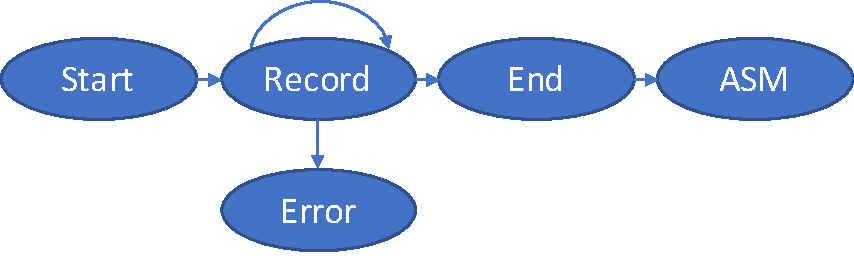
\includegraphics[width=\textwidth]{luajit/images/chapter3/FSM.pdf}
    \caption{Recorder state machine}
    \label{fig:recorder-state-machine}
\end{figure}


\begin{table}[H]
\centering
\caption{States description}
\label{tab:states}
\begin{tabularx}{\textwidth}{|c|X|}
\hline
\multicolumn{1}{|c|}{States}          & \multicolumn{1}{c|}{Description}                     \\\hline
Start                   &
  \begin{tabular}[c]{@{}l@{}}
  Call trace\_start that perform jit\_State setup and \\allocations.
  Change state to LJ\_TRACE\_RECORD.
  \end{tabular}                                                                             \\\hline
Record                  & Recording in progress. It loop over the
	lj\_record\_ins function, which is a huge switch case that record a specific
  bytecode instruction and generate the corresponding specialized IR code of the
  BC before execution. It is executed inside a pcall and jump to the
  \emph{Error} state if a Lua exception is thrown. \\\hline%
End                     &
  End of recording. It applies optimizations on the IR (see Chapter \ref{Sec:TO}).        \\\hline
ASM                     &
	Assemble the trace and call trace\_stop to patch the BC (see Chapter \ref{Sec:TA}).     \\\hline
Error                   &
	Abort the recording of the current trace, perform state cleanup, penalize the
	corresponding hot BC or apply blacklisting (see Section \ref{Subsec:abort})                  \\\hline
\end{tabularx}
\end{table}

%===============================================================================
% Abortion and blacklisting
%===============================================================================

\subsection{Abortion and blacklisting}
\label{Subsec:abort}

There exist multiple reason that might cause a recording to abort such as
the unroll limit is reached, the trace is too long, the
JIT is disabled for a specific function or many others (see \emph{lj\_traceerr.h}
for the list of possible abort messages). To trigger an abortion, a Lua error is
thrown during the recording which transition the recorder state machine to the
\emph{LJ\_TRACE\_ERR} state. Then, the \emph{penalty\_pc} function is called on
the hot bytecode that triggered the recording. The penalty mechanism consists of
a 64-entry table, where each entry is a structure containing the exact PC of the
penalized bytecode, the penalty value, and the reason of the abortion. The
\emph{penaltyslot} variable is a round-robin index inside the table indicating
the next entry to use if a new bytecode needs to be penalized. It as to be noted
that on the contrary of the hotcount mechanism, here the full PC is used to
identify a slot making false positive impossible. However, since the entry is
only 64 entry, penalized bytecode can easily be forgotten in a big code base.
If the penalty of a bytecode exceeds a threshold then the hot bytecode
responsible for starting the recording gets blacklisted. It means that this
bytecode can never become hot again and start a recording. It also means that if this
bytecode try to be recorded inside another trace, this trace get aborted too
(in most cases). A blacklisted bytecode is never whitelisted by the system.

%===============================================================================
% Intermediate representation
%===============================================================================

\subsection{Intermediate representation}
\label{Subsec:IR}

LuaJIT use a single high-level intermediate representation (IR) across all
optimization stage. As stated, it is generated on the fly during recording and
it is SSA based (static single assignment). It is implemented with a
bidirectional growable array in memory. It includes two different things:
instructions and constants. Instructions are stored at positive indices, while
constants are stored at negative indices. IR references are 16-bits index inside
the IR array and are biased by adding 0x8000 (negative indices are $<$ 0x8000).
All constants are interned and can be compared for equality only by looking at
their references, simplifying many optimization algorithm. Every instruction has
an output data type. Since the Control-flow is flattened, it is always implicit.
Data-flow for loops is represented using PHI-instructions. Other types of
control-flows are managed using guarded instructions. If a guarded instruction
succeeds the normal execution proceed, otherwise the trace is exited. Those
instructions have two purposes, they are generated by the backend to represent
Lua branching code and they are used as assertions on operands to test the
validity of assumptions made during recording. If a trace exit is taken the VM
states are restored using the last snapshot (See Section \ref{Subsec:snap}). If a trace exit is taken a
sufficient number of times, a child trace is recorded
(trace starting from the exit of a parent trace). Remember that side traces are
not recursive (a side trace cannot have a side trace). The IR is threaded with
segregated, per-opcode skip-list chains. The links are stored in the \emph{prev}
field in the instruction (see Table below). This facilitates low-overhead
lookup for many IR optimizations (i.e. CSE, DSE and alias analysis).

\begin{table}[H]
\centering
\caption{IR instruction format (64 bit)}
\label{tab:ir-format}
\begin{tabular}{|l|c|c|c|c|c|c|}
\hline
\multicolumn{1}{|c|}{size}    & 16              & 16              & 8          & 8          & 8           & 8           \\ \hline
IR after register allocation  & op1             & op2             & t          & o          & r           & s           \\ \hline
IR before register allocation & \multicolumn{2}{c|}{op12/i/gco32} & \multicolumn{2}{c|}{ot} & \multicolumn{2}{c|}{prev} \\ \hline
Constants                     & \multicolumn{6}{c|}{TValue/gco64}                                                       \\ \hline
\end{tabular}
\end{table}

\begin{table}[H]
\centering
\caption{Field definitions.}
\label{tab:ir-field}
\begin{tabular}{|c|l|}
\hline
op1/2 & operands                    \\ \hline
t     & type                        \\ \hline
o     & opcode                      \\ \hline
r     & register allocation         \\ \hline
s     & spill slot                  \\ \hline
prev  & per-opcode skip-list chains \\ \hline
\end{tabular}
\end{table}

%===============================================================================
% Snapshots
%===============================================================================

\subsection{Snapshots}
\label{Subsec:snap}

Snapshot is an important mechanism used in trace compilation. The VM should
always be in a consistent state, meaning that all updates should respect the
original language semantics. However, to perform some trace optimization
(e.g. sinking optimization \ref{Subsec:opt-sinking}) this consistency is not respected. Instead
modification that should have occurred during a trace is recorded inside the
snapshots and those modifications are replayed at trace exit. The Snapshot
mechanism is implemented in the snap.[hc] files, and you can find the
\emph{SnapShot} data-structure in lj\_jit.h. For details about
Snapshot usages and implementation refer to section of the wiki on sinking
optimization \cite{luajit-sink} and a mail on the subject \cite{luajit-mail-1}.




%===============================================================================
% TRACE OPTIMIZER
%===============================================================================

\section{Trace optimizer}
\label{Sec:TO}
    
    
We can differentiate in the code, three types of optimizations.
First of all, there are the optimizations present in the optimization engine.
They are implemented in the \emph{lj\_opt\_*.c} files and thus easy to spot out.
Those optimization are of two kinds, global optimization that are run on the
entire IR at once at the end of the recording phase, during the
\emph{LJ\_TRACE\_END} state (See \ref{Subsec:opt-dce}, \ref{Subsec:opt-loop},
\ref{Subsec:opt-split}, \ref{Subsec:opt-sinking}) and the local optimizations
that are applied while recording a trace (See \ref{Subsec:narrowing},
\ref{Subsubsec:fold}, \ref{Subsubsec:mao}). Finally, there is a plethora of
optimization and heuristic applied here and there (See LuaJIT wiki on
optimization \cite{luajit-opt}).

%===============================================================================
% Dead code elimination
%===============================================================================

\subsection{Dead code elimination}
\label{Subsec:opt-dce}

DCE or Dead Code Elimination is performed by the lj\_opt\_dce main function
in two phases. During the first phase called mark snap, it mark all IR
instructions that are referenced by a snapshot. The second phases called
propagate, iteratively mark all IR instruction that are referenced by an already
marked IR instruction while replacing non-marked IR instruction by nops.

%===============================================================================
% Loop optimizations
%===============================================================================

\subsection{Loop optimizations}
\label{Subsec:opt-loop}

The loop optimization is a way to improve code hoisting for trace based on
loops. In fact LuaJIT should try to hoist most invariant instruction and guards
in such a way that trace that doesn't match the current dynamic profile of
the code (assumption on data or type) are exited as soon as possible.
Unfortunately due to the dynamic nature of the IR generated, it contains many
guards and thus are control-dependent, making little room for loop-invariant
code motion (LICM). The solution used here is a copy-substitution of the body
of the loop. It basically consists in always unrolling the loop once before the
actual loop instruction. This allows the code executed inside the loop to
contains only variant instructions.

%===============================================================================
% Split optimizations
%===============================================================================

\subsection{Split optimizations}
\label{Subsec:opt-split}

The split optimization is only used by 32-bits architecture and splits the
64-bits IR instructions into multiple 32-bits once.

%===============================================================================
% Sinking optimizations
%===============================================================================

\subsection{Sinking optimizations}
\label{Subsec:opt-sinking}
This is a very useful optimization that allows to avoid many temporaries and
unnecessary memory accesses and allocations by keeping the values of interest
directly in register. Since memory modifications are not performed, we need a way
to remember the writes in case those value escape the execution path
(are not temporary anymore). For this purpose snapshots are used (See Section \ref{Subsec:snap}).
This optimization is implemented in the \emph{lj\_opt\_sink.c} file. A detailed
explanation of this optimization is available on the wiki \cite{luajit-sink}.

%===============================================================================
% Narrowing optimizations
%===============================================================================

\subsection{Narrowing optimizations}
\label{Subsec:narrowing}

It performs the narrowing of Lua numbers (double) into integers when it seems
to be useful. LuaJIT use demand-driven (by the backend) narrowing for index
expressions, integer arguments (FFI), and bit operations and predictive
narrowing for induction variables. It emits overflow check instruction when
necessary. Most arithmetic operations are never narrowed. To learn more on why,
see the comment section in the \emph{lj\_opt\_narrow.c} file.

%===============================================================================
% Fold engine
%===============================================================================

\subsection{Fold engine}
\label{Subsec:fold}

The fold engine implement a rule-based mechanism. Rules are declared using the
LJFOLD macro which contains the IR opcode and a rule on the parameters it
applies to. During the LuaJIT buildvm (more precisely the \emph{buildvm\_fold.c}
file) those rules are scanned and the \emph{lj\_foldef.h} file gets generated.
It contains a semi-perfect hash table for constant-time rule lookups, where each
entry respect the format depicted in Table \ref{tab:fold-format}. It also
contains a second table containing the function to call if a corresponding rule
match.

\begin{table}[H]
\centering
\caption{Fold hash table, bit pattern entry}
\label{tab:fold-format}
\begin{tabular}{|c|c|c|c|c|}
\hline
8 bits           & 7 bits            & 7 bits            & 2 bits   & 8 bits                      \\ \hline
index fold table & fold instr opcode & left instr opcode & 00       & right instr opcode      \\ \hline
index fold table & fold instr opcode & left instr opcode & \multicolumn{2}{c|}{literal field} \\ \hline
\end{tabular}
\end{table}

\subsubsection{Fold optimizations}
\label{Subsubsec:fold}

The fold optimizations preformed by the FOLD engine are implemented in the
\emph{lj\_opt\_fold.c} file and can be separated in five well-known techniques,
constant folding, algebraic simplifications, reassociation, common subexpression
elimination and array bounds check elimination.

\subsubsection{Memory access optimizations}
\label{Subsubsec:mao}

The memory access optimization perform by the FOLD engine and implemented
in the lj\_opt\_mem.c file consists of three components, the alias
analysis using high-level semantic disambiguation, Load to load and store to load
forwarding, and finally dead-store elimination.


%===============================================================================
%   ASSEMBLER
%===============================================================================

\section{Assembler}
\label{Sec:TA}

When the recorder state machine reaches the \emph{LJ\_TRACE\_ASM} state, the
\emph{lj\_asm\_trace} main assembler function is called. This function is
responsible for the setup and teardown of the assembler phase. Each IR
instruction of the trace is assembled through the \emph{asm\_ir} function which
is a switch case on the opcode. The implementation of the assembler is divided
in three different files. \emph{lj\_asm.c} contains the assembler code that is
agnostic of the platform, \emph{lj\_asm\_(target).h} contains the assembler code
specific to a particular target (i.e. x86), and \emph{lj\_emit\_(target).h}
contain the helper functions for generating instructions for a specific
instruction-set. A trace is assembled in linear, backwards order. It uses
\emph{ASMState} has the main data structure that helps with, physical register
allocation, machine code and IR traversal, and snapshots handling. At the end of
the assembler phase, the bytecode is patched to circumvent the following bytecodes
and call the compiled trace instead.

% -- TO BE ADDED ????
% in lj_trace.c ? (verify)
% - lj_record_stop
%   - trace stitching (call to C using C API)
%   - end of the hotloop
%   - hit an other already compiled loop (link to it)
%   - return statement
%     - return to interpretor for unhandled cases
%     - when downrec limit reach for side-trace (nagative frame depth)
%     - tail-rec is detected (limit reach in the same framedepth)
%     - limit reach in up recursion (positive frame depth)
%   - hit a compiled function (link to its trace)
    
    
